\chapter{Elements}

A lattice for a storage ring or linac is made up of a collection of
elements --- quadrupoles, bends, etc. This chapter discusses the
various types of elements available in \bmad\ except for \vn{group}s
and \vn{overlay}s which are discussed in the next chapter.

\section{Bmad Elements}

Most element types available in \mad\ are provided in \bmad.
Additionally, \bmad\ provides a number of element types that are not
available in \mad.  A word of caution: In some cases where both \mad\
and \bmad\ provide the same element type, there will be an overlap of 
the attributes available but the two sets of attributes will not be the same.
The list of element types known to \bmad\ is shown in Table~\ref{tab:elements}.
In
\begin{table}[h]
\centering
{\tt
\begin{tabular}{|l|l||l|l|} \hline
  {\it Element} & {\it Section}     & {\it Element} & {\it Section}    \\ \hline
  AB\_Multipole & \ref{s:ab_m}      &  Octupole     & \ref{s:oct}      \\ \hline
  Accel\_Sol    & \ref{s:accel_sol} &  Overlay      & \ref{s:overlay}  \\ \hline
  BeamBeam      & \ref{s:bbi}       &  Patch        & \ref{s:patch}    \\ \hline
  Custom        & \ref{s:custom}    &  Quadrupole   & \ref{s:quad}     \\ \hline
  Drift         & \ref{s:drift}     &  Rbend        & \ref{s:bend}     \\ \hline
  Ecollimator   & \ref{s:col}       &  Rcollimator  & \ref{s:col}      \\ \hline
  ElSeparator   & \ref{s:elsep}     &  RFcavity     & \ref{s:rfcav}    \\ \hline
  Group         & \ref{s:group}     &  Sbend        & \ref{s:bend}     \\ \hline
  HKicker       & \ref{s:hvkicker}  &  Sextupole    & \ref{s:sex}      \\ \hline
  Hybrid        & \ref{s:hybrid}    &  Solenoid     & \ref{s:sol}      \\ \hline
  Instrument    & \ref{s:monitor}   &  Sol\_Quad    & \ref{s:sq}       \\ \hline
  Kicker        & \ref{s:kicker}    &  Taylor       & \ref{s:tay}      \\ \hline
  LCavity       & \ref{s:lcav}      &  VKicker      & \ref{s:hvkicker} \\ \hline
  Marker        & \ref{s:mark}      &  Wiggler      & \ref{s:wig}      \\ \hline
  Monitor       & \ref{s:monitor}   &               &                  \\ \hline
  Multipole     & \ref{s:mult}      &               &                  \\ \hline
\end{tabular}
}
\caption{\bmad\ elements.}
\label{tab:elements}\center
\end{table}

\vfil
\break

%-----------------------------------------------------------------
\section{AB\_Multipole}
\label{s:ab_m}

An \vn{AB_Multipole} is a thin multipole lens up to 20th order. The only
difference between this and a \vn{Multipole} is the input format. See the 
Magnetic fields section \ref{s:fields} for more details.

\toffset
\begin{center}
\tt 
\begin{tabular}{|l|l||l|l||l|l|} \hline
  {\sl Attribute} & {\sl Sec.}  & {\sl Attribute} & {\sl Sec} & {\sl Attribute} & {\sl Sec.} \\ \hline
  a$n$, b$n$ = Real  &  \ref{s:fields} &  type = String    & \ref{s:string} & tracking\_method = Switch    & \ref{s:tkm}   \\ \hline
  tilt       = Real  &  \ref{s:offset} &  alias = String   & \ref{s:string} & mat6\_calc\_method = Switch  & \ref{s:xfer}  \\ \hline
  x\_offset  = Real  &  \ref{s:offset} &  descrip = String & \ref{s:string} & x\_limit = Real              & \ref{s:limit} \\ \hline
  y\_offset  = Real  &  \ref{s:offset} &  is\_on = Logical & \ref{s:is_on}  & y\_limit = Real              & \ref{s:limit} \\ \hline
  s\_offset  = Real  &  \ref{s:offset} &                   &                & aperture = Real              & \ref{s:limit} \\ \hline
\end{tabular}
\end{center}
\toffset

Unlike a \mad\ \vn{multipole}, An \vn{AB_Multipole} never affects the
reference orbit even if there is a dipole component. For \vn{a$n$},
and \vn{b$n$} $n$ is in the range 0 through 20.

\vskip0.05in \noindent
Example:
\begin{example}
  abc: ab_multipole, a2 = 0.034e-2, b3 = 5.7, a11 = 5.6e6/2
\end{example}

\vskip0.05in \noindent
Dependent attributes:
\begin{example}
  beam\_energy  ! See section \ref{s:beam}
\end{example}

%-----------------------------------------------------------------
\section{Accel\_Sol}
\label{s:accel_sol}

An \vn{Accel_Sol} element is a combination LINAC RF accelerating
section with a solenoid on top of it. For historical reasons this
element is not currently available but could be revived if there is
any demand for it.

%-----------------------------------------------------------------
\section{BeamBeam}
\label{s:bbi}

A \vn{BeamBeam} element simulates an interaction with an opposing
(``strong'') beam traveling in the opposite direction (a
``weak--strong beam--beam Interaction''). The strong beam is assumed
to be Gaussian in shape.

\toffset
\begin{center} 
\tt
\begin{tabular}{|l|l||l|l||l|l|} \hline
  {\sl Attribute} & {\sl Sec.}  & {\sl Attribute} & {\sl Sec.} & {\sl Attribute} & {\sl Sec.} \\ \hline
  sig\_x   = Real       &                 & type = String    & \ref{s:string} & tracking\_method = Switch    & \ref{s:tkm}    \\ \hline
  sig\_y   = Real       &                 & alias = String   & \ref{s:string} & mat6\_calc\_method = Switch  & \ref{s:xfer}   \\ \hline
  sig\_z   = Real       &                 & descrip = String & \ref{s:string} &                              &                \\ \hline
  charge   = Real       &                 & x\_pitch = Real  & \ref{s:offset} & x\_offset  = Real            & \ref{s:offset} \\ \hline
  n\_slice = Integer    &                 & y\_pitch = Real  & \ref{s:offset} & y\_offset  = Real            & \ref{s:offset} \\ \hline
  x\_limit = Real       & \ref{s:limit}   & tilt = Real      & \ref{s:offset} & s\_offset  = Real            & \ref{s:offset} \\ \hline
  y\_limit = Real       & \ref{s:limit}   & is\_on = Logical & \ref{s:is_on}  & symplectify = Logical        & \ref{s:symp}   \\ \hline
  aperture = Real       & \ref{s:limit}   &                  &                &                              &                \\ \hline
\end{tabular}
\end{center}
\toffset

The magnitude of the strong beam's charge is set by the \vn{beam}
command (see \ref{s:beam}).  The sign of the strong beam's charge is
set by the \vn{charge} attribute. If \vn{charge} = -1 the
strong beam has the opposite charge. This is the default.

\vn{sig_x}, \vn{sig_y}, \vn{sig_z} are the strong beam sigmas. 
In \bmad, \vn{x_offset} and \vn{y_offset} are used to offset the
\vn{BeamBeam} element instead of the \mad\ standard attributes
\vn{xma} and \vn{yma}.

\vn{x_pitch} and \vn{y_pitch} gives the beam--beam interaction a
crossing angle. This is the full crossing angle, not the half-angle.

The strong beam is divided up into \vn{n_slice} equal charge (not equal
thickness) slices. The default for \vn{n_slice} is 1. Propagation
through the strong beam involves a kick at the charge center of each
slice with drifts in between the kicks. The kicks are calculated using
the standard Bassetti--Erskine formula.  Even though the strong beam can
have a finite \vn{sig_z} the length of the element is always considered
to be zero. This is achieved by adding drifts at either end of any
tracking so that the starting point and ending point are
identical. The longitudinal $s$--position of the
\vn{BeamBeam} element is at the spot where the reference particle's
position coincides with the center of the strong bunch. For example,
with \vn{n_slice} = 2 the calculation would proceed as follows:
\begin{example}
  0) Start with the reference particle at the center of the strong bunch.
  1) Propagate (drift) backwards to the center of the first slice.
  2) Apply the beam--beam kick due to the first slice.
  3) Propagate (drift) forwards to the center of the second slice.
  4) Apply the beam--beam kick due to the second slice.
  5) Propagate (drift) backwards to end up with the reference particle
     at the center of the strong bunch.
\end{example}

\vskip0.05in \noindent
Example:
\begin{example}
  bbi: beambeam, sig\_x = 3e-3, sig\_y = 3e-4, x\_offset = 0.05
\end{example}

\vskip0.05in \noindent
Dependent attributes:
\begin{example}
  beam\_energy  ! See section \ref{s:beam}
  bbi\_constant 
\end{example}
\vn{bbi_constant}: $ C_{bbi} = 
N \, m_e \, r_e / (2 \, \pi \, \gamma \, (\sigma_x + \sigma_y))$ 
is a measure of the beam--beam interaction strength. For example,
in the linear region near $x = y = 0$ the horizontal component of the
beam--beam kick is approximately 
$k_x = -4\, \pi \, x \, C_{bbi} / \sigma_x$ and the
horizontal beam--beam tune shift is 
$dQ_x = C_{bbi} \, \beta_x / \sigma_x$.

%-----------------------------------------------------------------
\section{Custom}
\label{s:custom}

A \vn{Custom} element is an element whose properties are defined
outside of the standard \bmad\ subroutine library. That is, to use a
custom element some programmer must write the appropriate custom
routines which are then linked with the \bmad\ subroutines into a
program. \bmad\ will call the custom routines at the appropriate time
to do tracking, transfer matrix calculations, etc. See the programmer
who wrote the custom routines for more details!

\toffset
\begin{center}
\tt
\begin{tabular}{|l|l||l|l||l|l|} \hline
  {\sl Attribute} & {\sl Sec.}  & {\sl Attribute} & {\sl Sec.} & {\sl Attribute} & {\sl Sec.} \\ \hline
  l        = Real              & \ref{s:l}      & type = String      & \ref{s:string} & tracking\_method = Switch   & \ref{s:tkm}   \\ \hline
  \begin{tabular}{@{}l} val$n$ = Real \\ ($n = 1 - 12$) \end{tabular} 
                               &                & alias = String     & \ref{s:string} & mat6\_calc\_method = Switch & \ref{s:xfer}  \\ \hline
  x\_offset  = Real            & \ref{s:offset} & descrip = String   & \ref{s:string} & integration\_ord = Integer  & \ref{s:integ} \\ \hline
  y\_offset  = Real            & \ref{s:offset} &                    &                & field\_calc = Switch        & \ref{s:integ} \\ \hline
  s\_offset  = Real            & \ref{s:offset} & is\_on             & \ref{s:is_on}  & rel\_tol = Real             & \ref{s:integ} \\ \hline
  x\_pitch = Real              & \ref{s:offset} & x\_limit = Real    & \ref{s:limit}  & abs\_tol = Real             & \ref{s:integ} \\ \hline
  y\_pitch = Real              & \ref{s:offset} & y\_limit = Real    & \ref{s:limit}  & num\_steps = Integer        & \ref{s:integ} \\ \hline
  tilt     = Real              & \ref{s:offset} & aperture = Real    & \ref{s:limit}  & symplectify = Logical       & \ref{s:symp}  \\ \hline
\end{tabular}
\end{center}
\toffset

\noindent
Example:
\begin{example}
  c1: custom, l = 3, val4 = 5.6, val12 = 0.9, num_steps = 12, tracking_method = boris
\end{example}

\vskip0.05in \noindent
Dependent attributes:
\begin{example}
  beam\_energy  ! See section \ref{s:beam}
\end{example}

%-----------------------------------------------------------------
\section{Drift}
\label{s:drift}

A \vn{Drift} element is just a space free and clear.

\toffset
\begin{center}
\tt
\begin{tabular}{|l|l||l|l||l|l|} \hline
  {\sl Attribute} & {\sl Sec.}  & {\sl Attribute} & {\sl Sec.} & {\sl Attribute} & {\sl Sec.} \\ \hline
  l        = Real       & \ref{s:l}     & type = String      & \ref{s:string} & tracking\_method = Switch    & \ref{s:tkm}   \\ \hline
                        &               & alias = String     & \ref{s:string} & mat6\_calc\_method = Switch  & \ref{s:xfer}  \\ \hline
  rel\_tol = Real       & \ref{s:integ} & descrip = String   & \ref{s:string} &                              &               \\ \hline
  abs\_tol = Real       & \ref{s:integ} & x\_limit = Real    & \ref{s:limit}  & symplectify = Logical        & \ref{s:symp}  \\ \hline
  num\_steps = Integer  & \ref{s:integ} & y\_limit = Real    & \ref{s:limit}  & integration\_ord = Integer   & \ref{s:integ} \\ \hline
                        &               & aperture = Real    & \ref{s:limit}  & field\_calc = Switch         & \ref{s:integ} \\ \hline
\end{tabular}
\end{center}
\toffset

\noindent
Example:
\begin{example}
  d21: drift, l = 4.5
\end{example}

\vskip0.05in \noindent
Dependent attributes:
\begin{example}
  beam\_energy  ! See section \ref{s:beam}
\end{example}

%-----------------------------------------------------------------
\section{Ecollimator and Rcollimator}
\label{s:col}

An \vn{Ecollimator} is a drift with elliptic collimation.
A \vn{Rcollimator} is a drift with rectangular collimation.
The aperture is considered to be at the end edge of the element.

\toffset
\begin{center}
\tt
\begin{tabular}{|l|l||l|l||l|l|} \hline
  {\sl Attribute} & {\sl Sec.}  & {\sl Attribute} & {\sl Sec.} & {\sl Attribute} & {\sl Sec.} \\ \hline
  l        = Real       & \ref{s:l}      & type = String                & \ref{s:string} & tracking\_method = Switch    & \ref{s:tkm}   \\ \hline
  num\_steps = Integer  & \ref{s:integ}  & alias = String               & \ref{s:string} & mat6\_calc\_method = Switch  & \ref{s:xfer}  \\ \hline
  rel\_tol = Real       & \ref{s:integ}  & descrip = String             & \ref{s:string} &                              &               \\ \hline
  abs\_tol = Real       & \ref{s:integ}  & x\_limit = Real              & \ref{s:limit}  & symplectify = Logical        & \ref{s:symp}  \\ \hline
  x\_offset  = Real     & \ref{s:offset} & y\_limit = Real              & \ref{s:limit}  & integration\_ord = Integer   & \ref{s:integ} \\ \hline
  y\_offset  = Real     & \ref{s:offset} & aperture = Real              & \ref{s:limit}  & field\_calc = Switch         & \ref{s:integ} \\ \hline                                
\end{tabular}
\end{center}
\toffset

\vskip0.05in \noindent
Example:
\begin{example}
  d21: ecollimator, l = 4.5, x_limit = 0.09/2, y_limit = 0.05/2
\end{example}

\vskip0.05in \noindent
Dependent attributes:
\begin{example}
  beam\_energy  ! See section \ref{s:beam}
\end{example}

%-----------------------------------------------------------------
\section{Elseperator}
\label{s:elsep}

A \vn{ElSeperator} is an electrostatic separator.

\toffset
\begin{center}
\tt
\begin{tabular}{|l|l||l|l||l|l|} \hline
  {\sl Attribute} & {\sl Sec.}  & {\sl Attribute} & {\sl Sec.} & {\sl Attribute} & {\sl Sec.} \\ \hline
  l        = Real       & \ref{s:l}      & type = String      & \ref{s:string} & tracking\_method = Switch   & \ref{s:tkm}   \\ \hline
  hkick    = Real       & \ref{s:kick}   & alias = String     & \ref{s:string} & mat6\_calc\_method = Switch & \ref{s:xfer}  \\ \hline
  vkick    = Real       & \ref{s:kick}   & descrip = String   & \ref{s:string} & integration\_ord = Integer  & \ref{s:integ} \\ \hline
  gap      = Real       &                &                    &                & field\_calc = Switch        & \ref{s:integ} \\ \hline
  x\_offset  = Real     & \ref{s:offset} & is\_on             & \ref{s:is_on}  & rel\_tol = Real             & \ref{s:integ} \\ \hline
  y\_offset  = Real     & \ref{s:offset} & x\_limit = Real    & \ref{s:limit}  & abs\_tol = Real             & \ref{s:integ} \\ \hline
  s\_offset  = Real     & \ref{s:offset} & y\_limit = Real    & \ref{s:limit}  & num\_steps = Integer        & \ref{s:integ} \\ \hline
  x\_pitch = Real       & \ref{s:offset} & aperture = Real    & \ref{s:limit}  & symplectify = Logical       & \ref{s:symp}  \\ \hline
  y\_pitch = Real       & \ref{s:offset} &                    &                & a$n$, b$n$ = Real           & \ref{s:fields}\\ \hline
  tilt     = Real       & \ref{s:offset} &                    &                & radius = Real               & \ref{s:fields}\\ \hline
\end{tabular}
\end{center}
\toffset

For an \vn{Elseparator}, the kick is determined by \vn{hkick} and
\vn{vkick}. The \vn{gap} for an \vn{Elseparator} is used to compute
the electric field for a given kick. The voltage is a dependent
attribute determined by:
\begin{example}
  e\_field (V/m) = sqrt(hkick^2 + vkick^2) * beam\_energy / L
  volt (V) = e\_field * gap  
\end{example}

\vskip0.05in \noindent
Example:
\begin{example}
  h_sep: elsep, l = 4.5, hkick = 0.003, gap = 0.11
\end{example}

\vskip0.05in \noindent
Dependent attributes:
\begin{example}
  beam\_energy  ! See section \ref{s:beam}
  e_field
  volt
\end{example}

%-----------------------------------------------------------------
\section{Hkicker and Vkicker}
\label{s:hvkicker}

A \vn{Hkicker} is a horizontal bend and a vn{Vkicker} is a vertical
bend.  Note that \vn{Hkicker} and \vn{Vkicker} elements use the
\vn{kick} attribute while a \vn{kicker} uses the \vn{hkick} and \vn{vkick} 
attributes.

\toffset
\begin{center}
\tt
\begin{tabular}{|l|l||l|l||l|l|} \hline
  {\sl Attribute} & {\sl Sec.} & {\sl Attribute} & {\sl Sec.} &  {\sl Attribute} & {\sl Sec.} \\ \hline
  l        = Real       & \ref{s:l}       & type = String      & \ref{s:string} & tracking\_method = Switch    & \ref{s:tkm}   \\ \hline
  kick     = Real       & \ref{s:kick}    & alias = String     & \ref{s:string} & mat6\_calc\_method = Switch  & \ref{s:xfer}  \\ \hline
  tilt     = Real       & \ref{s:offset}  & descrip = String   & \ref{s:string} & integration\_ord = Integer   & \ref{s:integ} \\ \hline
  rel\_tol = Real       & \ref{s:integ}   & x\_limit = Real    & \ref{s:limit}  & field\_calc = Switch         & \ref{s:integ} \\ \hline 
  abs\_tol = Real       & \ref{s:integ}   & y\_limit = Real    & \ref{s:limit}  & symplectify = Logical        & \ref{s:symp}  \\ \hline
  num\_steps = Integer  & \ref{s:integ}   & aperture = Real    & \ref{s:limit}  & is\_on                       & \ref{s:is_on} \\ \hline
\end{tabular}
\end{center}
\toffset

\vskip0.05in \noindent
Example:
\begin{example}
  h_kick: hkicker, l = 4.5, kick = 0.003
\end{example}

\vskip0.05in \noindent
Dependent attributes:
\begin{example}
  beam\_energy  ! See section \ref{s:beam}
\end{example}

%-----------------------------------------------------------------
\section{Hybrid}
\label{s:hybrid}

A \vn{Hybrid} element is an element that is formed by concatenating
other element together. \vn{Hybrid} elements are not part of the input
lattice file but are created by a program, usually for speed purposes.

%-----------------------------------------------------------------
\section{Instrument and Monitor}
\label{s:monitor}

\bmad\ treats \vn{Instrument} and \vn{Monitor} elements exactly like
a drift.

\toffset
\begin{center}
\tt
\begin{tabular}{|l|l||l|l||l|l|} \hline
  {\sl Attribute} & {\sl Sec.}  & {\sl Attribute} & {\sl Sec.} & {\sl Attribute} & {\sl Sec.} \\ \hline
  l        = Real       & \ref{s:l}     & type = String      & \ref{s:string} & tracking\_method = Switch    & \ref{s:tkm}   \\ \hline
                        &               & alias = String     & \ref{s:string} & mat6\_calc\_method = Switch  & \ref{s:xfer}  \\ \hline
  rel\_tol = Real       & \ref{s:integ} & descrip = String   & \ref{s:string} &                              &               \\ \hline
  abs\_tol = Real       & \ref{s:integ} & x\_limit = Real    & \ref{s:limit}  & symplectify = Logical        & \ref{s:symp}  \\ \hline
  num\_steps = Integer  & \ref{s:integ} & y\_limit = Real    & \ref{s:limit}  & integration\_ord = Integer   & \ref{s:integ} \\ \hline
                        &               & aperture = Real    & \ref{s:limit}  & field\_calc = Switch         & \ref{s:integ} \\ \hline
\end{tabular}
\end{center}
\toffset

\vskip0.05in \noindent
Example:
\begin{example}
  d21: instr, l = 4.5
\end{example}

\vskip0.05in \noindent
Dependent attributes:
\begin{example}
  beam\_energy  ! See section \ref{s:beam}
\end{example}

%-----------------------------------------------------------------
\section{Kicker}
\label{s:kicker}

A \vn{Kicker} can deflect a beam in both planes. Note that a
\vn{Kicker} uses the \vn{hkick} and \vn{vkick} attributes while
\vn{Hkicker} and \vn{Vkicker} elements use the \vn{kick} attribute. 
In addition a \vn{Kicker} can apply a displacement to a particle
using the \vn{h_displace} and \vn{v_displace} attributes.

\toffset
\begin{center}
\tt
\begin{tabular}{|l|l||l|l||l|l|} \hline
  {\sl Attribute} & {\sl Sec.} & {\sl Attribute} & {\sl Sec.} &  {\sl Attribute} & {\sl Sec.} \\ \hline
  l        = Real       & \ref{s:l}       & type = String      & \ref{s:string} & tracking\_method = Switch    & \ref{s:tkm}   \\ \hline
  hkick    = Real       & \ref{s:kick}    & alias = String     & \ref{s:string} & mat6\_calc\_method = Switch  & \ref{s:xfer}  \\ \hline
  vkick    = Real       & \ref{s:kick}    & descrip = String   & \ref{s:string} & integration\_ord = Integer   & \ref{s:integ} \\ \hline
  h\_displace = Real    &                 & x\_limit = Real    & \ref{s:limit}  & field\_calc = Switch         & \ref{s:integ} \\ \hline 
  v\_displace = Real    &                 & y\_limit = Real    & \ref{s:limit}  & symplectify = Logical        & \ref{s:symp}  \\ \hline
  rel\_tol = Real       & \ref{s:integ}   & aperture = Real    & \ref{s:limit}  & is\_on                       & \ref{s:is_on} \\ \hline
  abs\_tol = Real       & \ref{s:integ}   & tilt     = Real    & \ref{s:offset} &                              &               \\ \hline
  num\_steps = Integer  & \ref{s:integ}   &                    &                &                              &               \\ \hline
\end{tabular}
\end{center}
\toffset

\vskip0.05in \noindent
Example:
\begin{example}
  a_kick: kicker, l = 4.5, hkick = 0.003
\end{example}

\vskip0.05in \noindent
Dependent attributes:
\begin{example}
  beam\_energy  ! See section \ref{s:beam}
\end{example}

%-----------------------------------------------------------------
\section{Lcavity}
\label{s:lcav}

An \vn{Lcavity} is a LINAC accelerating cavity.

\toffset
\begin{center}
\tt
\begin{tabular}{|l|l||l|l||l|l|} \hline
  {\sl Attribute} & {\sl Sec.}  & {\sl Attribute} & {\sl Sec.} & {\sl Attribute} & {\sl Sec.} \\ \hline
  l        = Real       & \ref{s:l}      & type = String      & \ref{s:string} & tracking\_method = Switch   & \ref{s:tkm}   \\ \hline
  rf\_frequency = Real  &                & alias = String     & \ref{s:string} & mat6\_calc\_method = Switch & \ref{s:xfer}  \\ \hline
  gradient      = Real  &                & descrip = String   & \ref{s:string} & integration\_ord = Integer  & \ref{s:integ} \\ \hline
  phi0          = Real  &                &                    &                & field\_calc = Switch        & \ref{s:integ} \\ \hline
  e\_loss       = Real  &                & is\_on             & \ref{s:is_on}  & rel\_tol = Real             & \ref{s:integ} \\ \hline
  x\_offset  = Real     & \ref{s:offset} & x\_limit = Real    & \ref{s:limit}  & abs\_tol = Real             & \ref{s:integ} \\ \hline
  y\_offset  = Real     & \ref{s:offset} & y\_limit = Real    & \ref{s:limit}  & num\_steps = Integer        & \ref{s:integ} \\ \hline
  s\_offset  = Real     & \ref{s:offset} & aperture = Real    & \ref{s:limit}  &                             &               \\ \hline
  x\_pitch = Real       & \ref{s:offset} & hkick    = Real    & \ref{s:kick}   & sr\_wake\_file = String     &               \\ \hline
  y\_pitch = Real       & \ref{s:offset} & vkick    = Real    & \ref{s:kick}   & lr\_wake\_file = String     &               \\ \hline
\end{tabular}
\end{center}
\toffset

Tracking through an \vn{LCavity} is modeled using the equations developed by Rosenzweig
and Serafini\cite{b:rosenzweig}. The varias attributes are
\begin{example}
  gradient     ! Accelerating gradient in V/m
  phi0         ! Phase (in radians/2$pi$) of the reference particle with 
               !   respect to the RF. phi0 = 0 is on crest.
  e_loss       ! Loss parameter for short range wakefields in V/Coulomb.
  sr_wake_file ! Short range wake field definition file.
  lr_wake_file ! Long range wake field definition file.
\end{example}

The transfer matrix for an \vn{LCavity} with finite \vn{gradient} is never symplectic.

\vskip0.05in \noindent
Example:
\begin{example}
  rf1: lcav, l = 4.5, gradient = 1.2e6, sr\_wake\_file = "sr1.dat"
\end{example}

\vskip0.05in \noindent
Dependent attributes:
\begin{example}
  energy\_start
  beam\_energy  ! See section \ref{s:beam}
  e\_loss       ! If sr\_wake\_file is present
  delta\_e
\end{example}

%-----------------------------------------------------------------
\section{Marker}
\label{s:mark}

A \vn{Marker} is a zero length element meant to mark a position

\toffset
\begin{center}
\tt
\begin{tabular}{|l|l||l|l||l|l|} \hline
  {\sl Attribute} & {\sl Sec.}  & {\sl Attribute} & {\sl Sec.} & {\sl Attribute} & {\sl Sec.} \\ \hline
  tracking\_method = Switch    & \ref{s:tkm}  &  type = String      & \ref{s:string} & x\_limit = Real  & \ref{s:limit} \\ \hline 
  mat6\_calc\_method = Switch  & \ref{s:xfer} &  alias = String     & \ref{s:string} & y\_limit = Real  & \ref{s:limit} \\ \hline 
                               &              &  descrip = String   & \ref{s:string} & aperture = Real  & \ref{s:limit} \\ \hline 
\end{tabular}
\end{center}
\toffset

\vskip0.05in \noindent
Example:
\begin{example}
  mm: mark, type = "BPM"
\end{example}

\vskip0.05in \noindent
Dependent attributes:
\begin{example}
  beam\_energy  ! See section \ref{s:beam}
\end{example}

%-----------------------------------------------------------------
\section{Multipole}
\label{s:mult}

A \vn{Multipole} is a thin multipole lens up to 20th order. The only
difference between this and an \vn{AB_Multipole} is the input format. See the 
Magnetic fields section \ref{s:fields} for more details.

\toffset
\begin{center}
\tt
\begin{tabular}{|l|l||l|l||l|l|} \hline
  {\sl Attribute} & {\sl Sec}  & {\sl Attribute} & {\sl Sec} & {\sl Attribute} & {\sl Sec} \\ \hline
  K$n$L, T$n$ = Real &  \ref{s:fields} &  type = String                & \ref{s:string} & tracking\_method = Switch   & \ref{s:tkm}   \\ \hline
  tilt       = Real  &  \ref{s:offset} &  alias = String               & \ref{s:string} & mat6\_calc\_method = Switch & \ref{s:xfer}  \\ \hline
  x\_offset  = Real  &  \ref{s:offset} &  descrip = String             & \ref{s:string} & x\_limit = Real             & \ref{s:limit} \\ \hline
  y\_offset  = Real  &  \ref{s:offset} &  is\_on = Logical             & \ref{s:is_on}  & y\_limit = Real             & \ref{s:limit} \\ \hline
  s\_offset  = Real  &  \ref{s:offset} &                               &                & aperture = Real             & \ref{s:limit} \\ \hline
\end{tabular}
\end{center}
\toffset

Unlike \mad, A \vn{Multipole} never affects the reference orbit
even if there is a dipole (\vn{k0l}) component.

\vskip0.05in \noindent
Example:
\begin{example}
  m1: multipole, k1l = 0.034e-2, t1, k3l = 4.5, t3 = 0.31*pi
\end{example}

\vskip0.05in \noindent
Dependent attributes:
\begin{example}
  beam\_energy  ! See section \ref{s:beam}
\end{example}

%-----------------------------------------------------------------
\section{Octupole}
\label{s:oct}

An \vn{Octupole} has a cubic field dependence.

\toffset
\begin{center}
\tt
\begin{tabular}{|l|l||l|l||l|l|} \hline
  {\sl Attribute} & {\sl Sec.}  & {\sl Attribute} & {\sl Sec.} & {\sl Attribute} & {\sl Sec.} \\ \hline
  l        = Real       & \ref{s:l}      & type = String      & \ref{s:string} & tracking\_method = Switch   & \ref{s:tkm}   \\ \hline
  k3       = Real       &                & alias = String     & \ref{s:string} & mat6\_calc\_method = Switch & \ref{s:xfer}  \\ \hline
  b\_gradient = Real    &                & descrip = String   & \ref{s:string} & integration\_ord = Integer  & \ref{s:integ} \\ \hline
                        &                & is\_on             & \ref{s:is_on}  & field\_calc = Switch        & \ref{s:integ} \\ \hline
  x\_offset  = Real     & \ref{s:offset} & x\_limit = Real    & \ref{s:limit}  & rel\_tol = Real             & \ref{s:integ} \\ \hline
  y\_offset  = Real     & \ref{s:offset} & y\_limit = Real    & \ref{s:limit}  & abs\_tol = Real             & \ref{s:integ} \\ \hline
  s\_offset  = Real     & \ref{s:offset} & aperture = Real    & \ref{s:limit}  & num\_steps = Integer        & \ref{s:integ} \\ \hline
  x\_pitch = Real       & \ref{s:offset} & hkick    = Real    & \ref{s:kick}   & a$n$, b$n$ = Real           & \ref{s:fields}\\ \hline
  y\_pitch = Real       & \ref{s:offset} & vkick    = Real    & \ref{s:kick}   & radius = Real               & \ref{s:fields}\\ \hline
  tilt                  & \ref{s:offset} &                    &                & symplectify = Logical       & \ref{s:symp}  \\ \hline
\end{tabular}
\end{center}
\toffset

The \vn{Bmad_Standard} calculation treats an octupole using a kick--drift--kick model.


\vskip0.05in \noindent
Example:
\begin{example}
  oct1: octupole, l = 4.5, k3 = 0.003
\end{example}

\vskip0.05in \noindent
Dependent attributes:
\begin{example}
  beam\_energy  ! See section \ref{s:beam}
  b\_gradient or k3
\end{example}

%-----------------------------------------------------------------
\section{Patch}
\label{s:patch}

A \vn{Patch} offsets the reference orbit. This is a generalization of
\mad's \vn{yrot} and \vn{srot} elements. For example, a positive
\vn{x_offset} offsets the reference orbit after the \vn{patch} in the
positive $x$--direction relative to the reference orbit before the
\vn{patch}.

\toffset
\begin{center}
\tt
\begin{tabular}{|l|l||l|l||l|l|} \hline
  {\sl Attribute} & {\sl Sec}  & {\sl Attribute} & {\sl Sec} & {\sl Attribute} & {\sl Sec} \\ \hline
  x\_offset  = Real  & \ref{s:offset} &  type = String      & \ref{s:string} & tracking\_method = Switch   & \ref{s:tkm}   \\ \hline
  y\_offset  = Real  & \ref{s:offset} &  alias = String     & \ref{s:string} & mat6\_calc\_method = Switch & \ref{s:xfer}  \\ \hline
  z\_offset  = Real  & \ref{s:offset} &  descrip = String   & \ref{s:string} & x\_limit = Real             & \ref{s:limit} \\ \hline
  tilt = Real        & \ref{s:offset} &  x\_pitch   = Real  & \ref{s:offset} & y\_limit = Real             & \ref{s:limit} \\ \hline
                     &                &  y\_pitch   = Real  & \ref{s:offset} & aperture = Real             & \ref{s:limit} \\ \hline
                     &                &  de\_offset = Real  &                & is\_on = Logical            & \ref{s:is_on} \\ \hline
\end{tabular}
\end{center}
\toffset

\vskip0.in \noindent
Example:
\begin{example}
  pt: patch, x\_offset = 3.2
\end{example}

\vskip0.05in \noindent
Dependent attributes:
\begin{example}
  beam\_energy  ! See section \ref{s:beam}
\end{example}

%-----------------------------------------------------------------
\section{Quadrupole}
\label{s:quad}

An \vn{Quadrupole} has a linear field dependence.

\toffset
\begin{center}
\tt
\begin{tabular}{|l|l||l|l||l|l|} \hline
  {\sl Attribute} & {\sl Sec.}  & {\sl Attribute} & {\sl Sec.} & {\sl Attribute} & {\sl Sec.} \\ \hline
  l        = Real       & \ref{s:l}      & type = String      & \ref{s:string} & tracking\_method = Switch   & \ref{s:tkm}   \\ \hline
  k1       = Real       &                & alias = String     & \ref{s:string} & mat6\_calc\_method = Switch & \ref{s:xfer}  \\ \hline
  b\_gradient = Real    &                & descrip = String   & \ref{s:string} & integration\_ord = Integer  & \ref{s:integ} \\ \hline
                        &                & is\_on             & \ref{s:is_on}  & field\_calc = Switch        & \ref{s:integ} \\ \hline
  x\_offset  = Real     & \ref{s:offset} & x\_limit = Real    & \ref{s:limit}  & rel\_tol = Real             & \ref{s:integ} \\ \hline
  y\_offset  = Real     & \ref{s:offset} & y\_limit = Real    & \ref{s:limit}  & abs\_tol = Real             & \ref{s:integ} \\ \hline
  s\_offset  = Real     & \ref{s:offset} & aperture = Real    & \ref{s:limit}  & num\_steps = Integer        & \ref{s:integ} \\ \hline
  x\_pitch = Real       & \ref{s:offset} & hkick    = Real    & \ref{s:kick}   & a$n$, b$n$ = Real           & \ref{s:fields}\\ \hline
  y\_pitch = Real       & \ref{s:offset} & vkick    = Real    & \ref{s:kick}   & radius = Real               & \ref{s:fields}\\ \hline
  tilt     = Real       & \ref{s:offset} &                    &                & symplectify = Logical       & \ref{s:symp}  \\ \hline
\end{tabular}
\end{center}
\toffset

\vskip0.05in \noindent
Example:
\begin{example}
  q03w: quad, l = 0.6, k1 = 0.003, tilt
\end{example}

\vskip0.05in \noindent
Dependent attributes:
\begin{example}
  beam\_energy  ! See section \ref{s:beam}
  b\_gradient or k3
\end{example}

%-----------------------------------------------------------------
\section{Rbend and Sbend}
\label{s:bend}

\vn{Rbend} and \vn{Sbend} are dipole bends. The difference between
the two is the way the input attributes are interpreted.
\begin{figure}
  \centering
  \subfigure[rbend]
  {
    \label{rbend}
    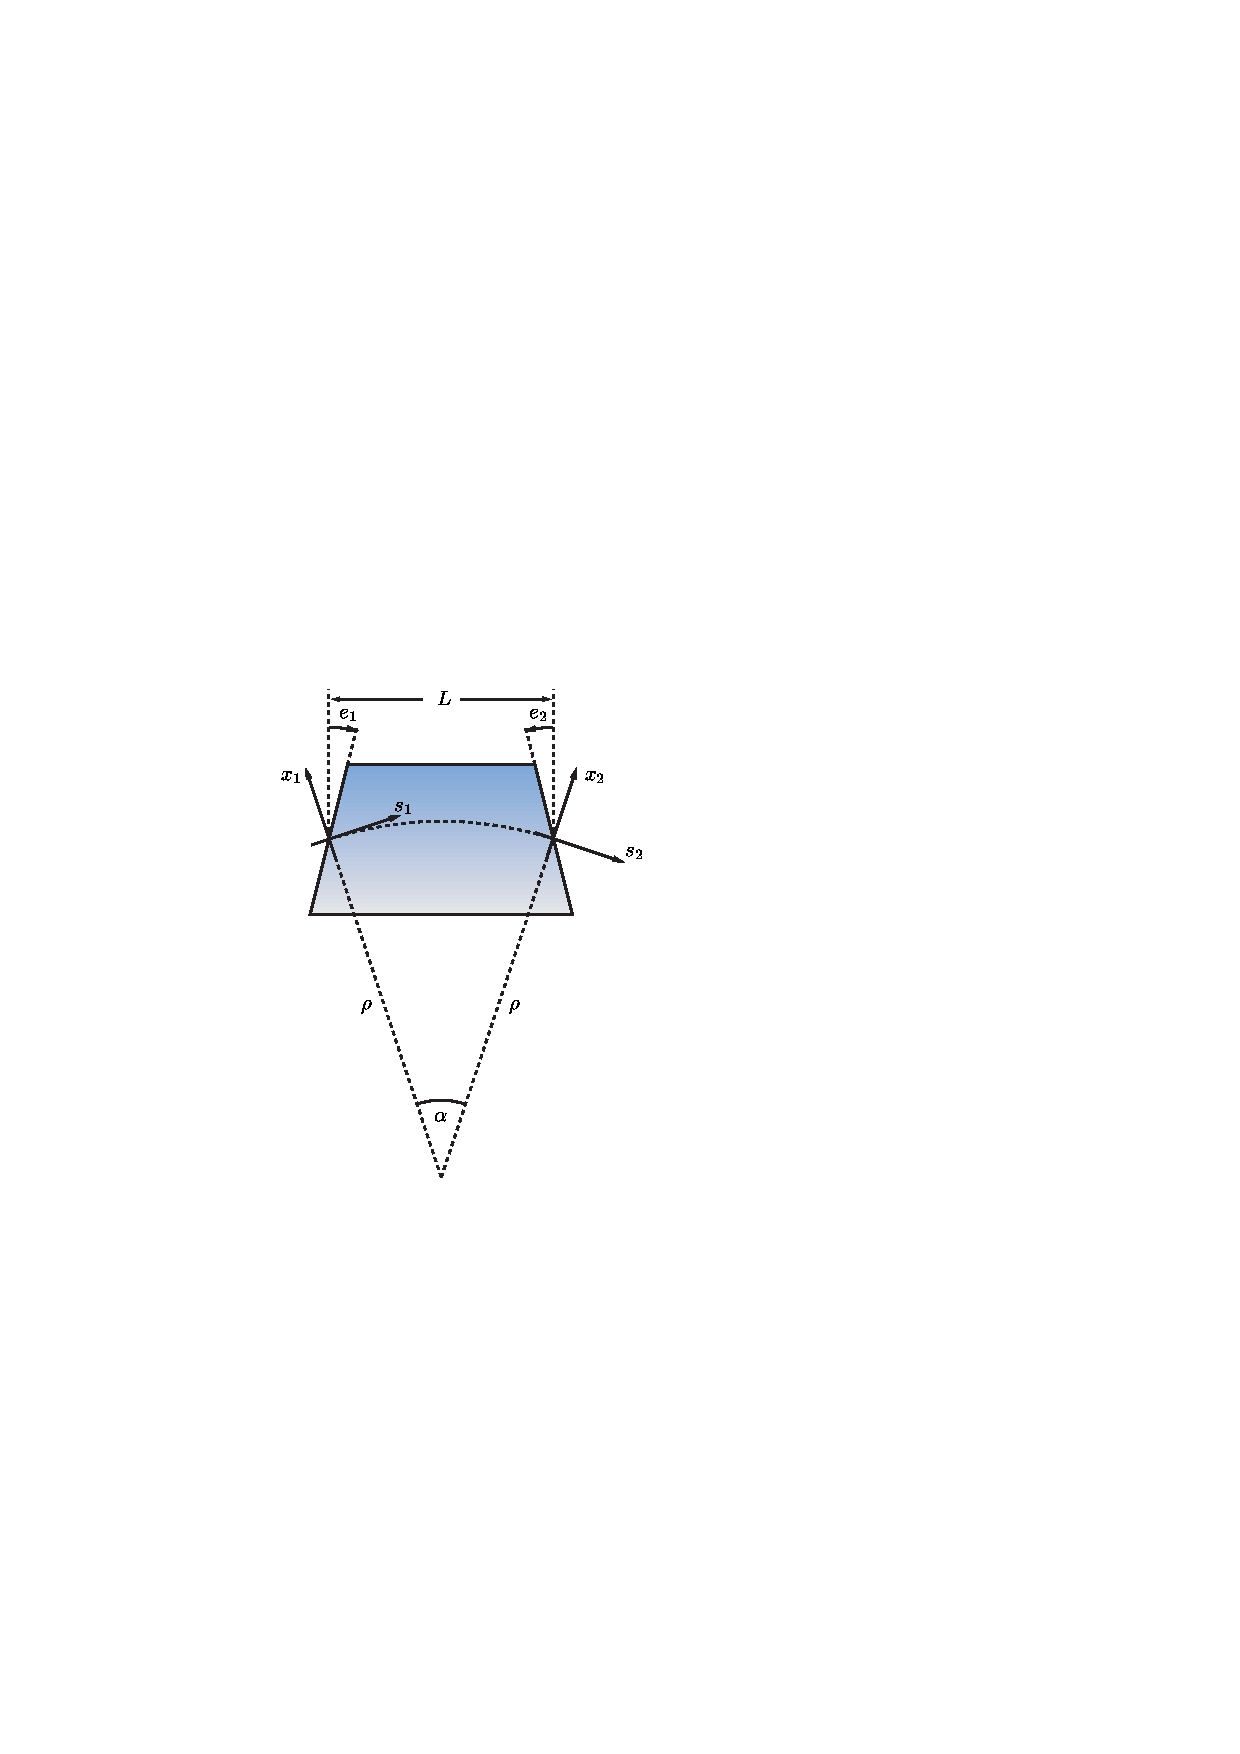
\includegraphics{rbend_coords.psfig}
  }
  \hspace{1cm}
  \subfigure[sbend]
  {
    \label{sbend}
    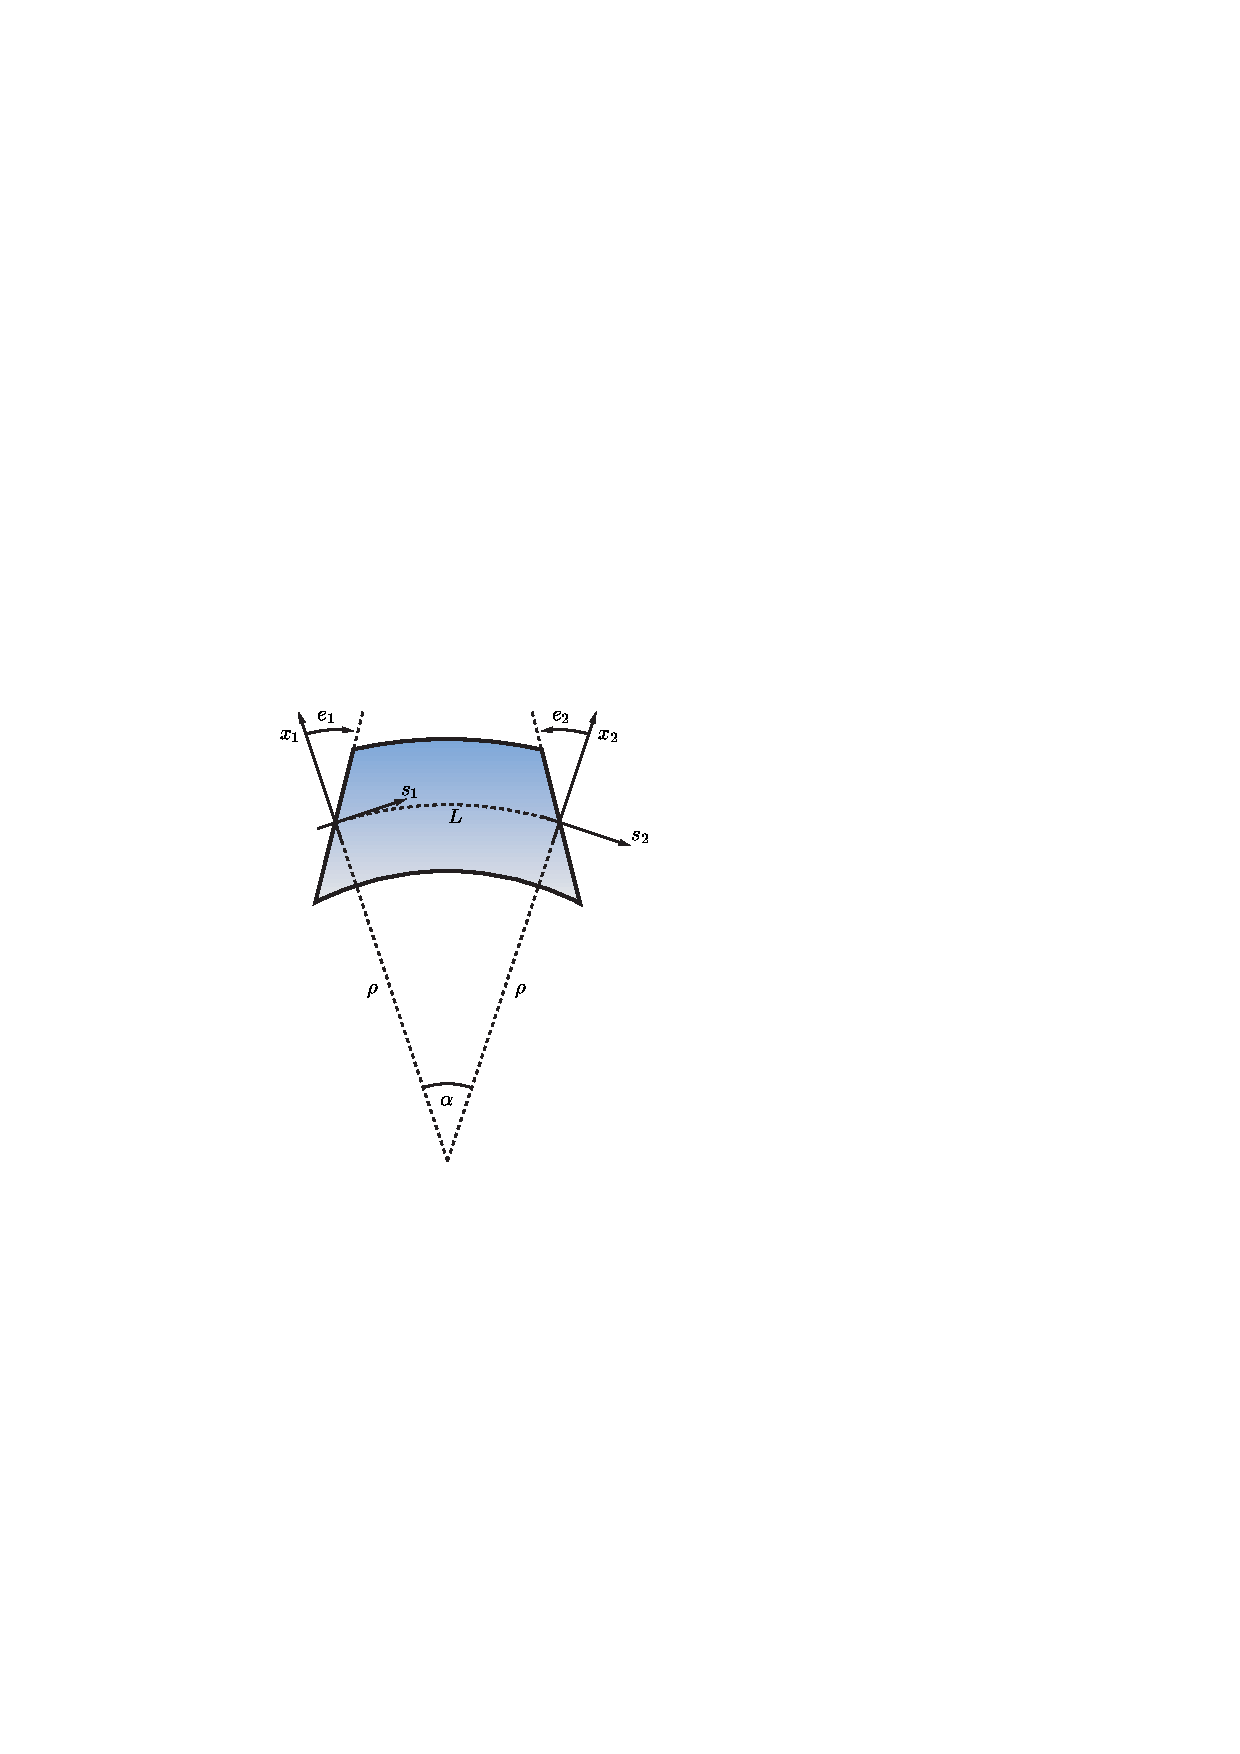
\includegraphics{sbend_coords.psfig}
  }
  \caption{Coordinate systems for rbend and sbend elements}
\end{figure}
  

\toffset
\begin{center}
\tt
\begin{tabular}{|l|l||l|l||l|l|} \hline
  {\sl Attribute} & {\sl Sec.}  & {\sl Attribute} & {\sl Sec.} & {\sl Attribute} & {\sl Sec.} \\ \hline
  l        = Real       & \ref{s:l}       & type = String      & \ref{s:string} & tracking\_method = Switch   & \ref{s:tkm}    \\ \hline
                        &                 & alias = String     & \ref{s:string} & mat6\_calc\_method = Switch & \ref{s:xfer}   \\ \hline
  g        = Real       &                 & descrip = String   & \ref{s:string} & x\_offset  = Real           & \ref{s:offset} \\ \hline
  delta\_g = Real       &                 &                    &                & y\_offset  = Real           & \ref{s:offset} \\ \hline
  e1       = Real       &                 &                    &                & s\_offset  = Real           & \ref{s:offset} \\ \hline
  e2       = Real       &                 & x\_limit = Real    & \ref{s:limit}  & x\_pitch = Real             & \ref{s:offset} \\ \hline
  b\_field = Real       &                 & y\_limit = Real    & \ref{s:limit}  & y\_pitch = Real             & \ref{s:offset} \\ \hline
  rho      = Real       &                 & aperture = Real    & \ref{s:limit}  & rel\_tol = Real             & \ref{s:integ}  \\ \hline
  angle    = Real       &                 & hkick    = Real    & \ref{s:kick}   & abs\_tol = Real             & \ref{s:integ}  \\ \hline
  tilt     = Real       & \ref{s:offset}  & vkick    = Real    & \ref{s:kick}   & num\_steps = Integer        & \ref{s:integ}  \\ \hline
  roll     = Real       & \ref{s:offset}  & fint     = Real    &                & integration\_ord = Integer  & \ref{s:integ}  \\ \hline
  k1       = Real       &                 & fintx    = Real    &                & field\_calc = Switch        & \ref{s:integ}  \\ \hline
  hgap     = Real       &                 & a$n$, b$n$ = Real  & \ref{s:fields} & symplectify                 & \ref{s:symp}   \\ \hline
  hgapx    = Real       &                 & radius = Real      & \ref{s:fields} & is\_on                      & \ref{s:is_on}  \\ \hline
\end{tabular}
\end{center}
\toffset

Note that \vn{l} for a \vn{RBend} is the chord length. Not the arc length as
it is for a \vn{SBend}.

After reading in a lattice, \bmad\ will internally convert all \vn{RBend}s
into \vn{SBend}s so \vn{l} will become the path length. The chord length will
be stored in the \vn{l_chord} attribute.

Use of \vn{hgap}, \vn{hgapx}, \vn{fint}, and \vn{fintx} is not yet implemented.

\vn{g}, \vn{angle}, and \vn{l} are mutually dependent. If any two are specified
for an element \bmad\ will calculate the appropriate value for the third.
After reading in a lattice \vn{angle} is considered a dependent variable.

For \vn{k1} = 0 \vn{Bmad_Standard} tracking does an exact geometrical 
calculation using thin quads at either end if there is non--zero edge
focusing.

\vskip0.05in \noindent
Example:
\begin{example}
  q03w: quad, l = 0.6, k1 = 0.003, tilt
\end{example}

\vskip0.05in \noindent
Dependent attributes:
\begin{example}
  beam\_energy  ! See section \ref{s:beam}
  b\_field or g
  rho
  angle
  l\_chord
\end{example}

%-----------------------------------------------------------------
\section{RFcavity}
\label{s:rfcav}

An \vn{RFcavity} is a RF cavity without acceleration generally used in a storage ring.

\toffset
\begin{center}
\tt
\begin{tabular}{|l|l||l|l||l|l|} \hline
  {\sl Attribute} & {\sl Sec.}  & {\sl Attribute} & {\sl Sec.} & {\sl Attribute} & {\sl Sec.} \\ \hline
  l        = Real       & \ref{s:l}      & type = String      & \ref{s:string} & tracking\_method = Switch   & \ref{s:tkm}   \\ \hline
  harmon   = Real       &                & alias = String     & \ref{s:string} & mat6\_calc\_method = Switch & \ref{s:xfer}  \\ \hline
  volt     = Real       &                & descrip = String   & \ref{s:string} & integration\_ord = Integer  & \ref{s:integ} \\ \hline
  phi0     = Real       &                &                    &                & field\_calc = Switch        & \ref{s:integ} \\ \hline
  x\_offset  = Real     & \ref{s:offset} & x\_limit = Real    & \ref{s:limit}  & rel\_tol = Real             & \ref{s:integ} \\ \hline
  y\_offset  = Real     & \ref{s:offset} & y\_limit = Real    & \ref{s:limit}  & abs\_tol = Real             & \ref{s:integ} \\ \hline
  s\_offset  = Real     & \ref{s:offset} & aperture = Real    & \ref{s:limit}  & num\_steps = Integer        & \ref{s:integ} \\ \hline
  x\_pitch = Real       & \ref{s:offset} & hkick    = Real    & \ref{s:kick}   & is\_on                      & \ref{s:is_on} \\ \hline
  y\_pitch = Real       & \ref{s:offset} & vkick    = Real    & \ref{s:kick}   & symplectify = Logical       & \ref{s:symp}  \\ \hline
\end{tabular}
\end{center}
\toffset


\vskip0.05in \noindent
Example:
\begin{example}
  rf1: lcav, l = 4.5, harmon = 1281, volt = 5e6
\end{example}

\vskip0.05in \noindent
Dependent attributes:
\begin{example}
  beam\_energy  ! See section \ref{s:beam}
  rf\_wavelength
\end{example}

%-----------------------------------------------------------------
\section{Sextupole}
\label{s:sex}
A \vn{Sextupole} has a quadratic field dependence.

\toffset
\begin{center}
\tt
\begin{tabular}{|l|l||l|l||l|l|} \hline
  {\sl Attribute} & {\sl Sec.}  & {\sl Attribute} & {\sl Sec.} & {\sl Attribute} & {\sl Sec.} \\ \hline
  l        = Real       & \ref{s:l}      & type = String      & \ref{s:string} & tracking\_method = Switch   & \ref{s:tkm}   \\ \hline
  k2       = Real       &                & alias = String     & \ref{s:string} & mat6\_calc\_method = Switch & \ref{s:xfer}  \\ \hline
  b\_gradient = Real    &                & descrip = String   & \ref{s:string} & integration\_ord = Integer  & \ref{s:integ} \\ \hline
                        &                & is\_on             & \ref{s:is_on}  & field\_calc = Switch        & \ref{s:integ} \\ \hline
  x\_offset  = Real     & \ref{s:offset} & x\_limit = Real    & \ref{s:limit}  & rel\_tol = Real             & \ref{s:integ} \\ \hline
  y\_offset  = Real     & \ref{s:offset} & y\_limit = Real    & \ref{s:limit}  & abs\_tol = Real             & \ref{s:integ} \\ \hline
  s\_offset  = Real     & \ref{s:offset} & aperture = Real    & \ref{s:limit}  & num\_steps = Integer        & \ref{s:integ} \\ \hline
  x\_pitch = Real       & \ref{s:offset} & hkick    = Real    & \ref{s:kick}   & a$n$, b$n$ = Real           & \ref{s:fields}\\ \hline
  y\_pitch = Real       & \ref{s:offset} & vkick    = Real    & \ref{s:kick}   & radius = Real               & \ref{s:fields}\\ \hline
  tilt     = Real       & \ref{s:offset} &                    &                & symplectify = Logical       & \ref{s:symp}  \\ \hline
\end{tabular}
\end{center}
\toffset

The \vn{Bmad_Standard} calculation treats a sextupole using a kick--drift--kick model.

\vskip0.05 in \noindent
Example:
\begin{example}
  q03w: quad, l = 0.6, k1 = 0.003, tilt
\end{example}

\vskip0.05in \noindent
Dependent attributes:
\begin{example}
  beam\_energy  ! See section \ref{s:beam}
  b\_gradiant or k3
\end{example}


%-----------------------------------------------------------------
\section{Solenoid}
\label{s:sol}

\toffset
\begin{center}
\tt
\begin{tabular}{|l|l||l|l||l|l|} \hline
  {\sl Attribute} & {\sl Sec.}  & {\sl Attribute} & {\sl Sec.} & {\sl Attribute} & {\sl Sec.} \\ \hline
  l        = Real       & \ref{s:l}      & type = String      & \ref{s:string} & tracking\_method = Switch   & \ref{s:tkm}   \\ \hline
  ks       = Real       &                & alias = String     & \ref{s:string} & mat6\_calc\_method = Switch & \ref{s:xfer}  \\ \hline
  b\_gradient = Real    &                & descrip = String   & \ref{s:string} & integration\_ord = Integer  & \ref{s:integ} \\ \hline
                        &                & is\_on             & \ref{s:is_on}  & field\_calc = Switch        & \ref{s:integ} \\ \hline
  x\_offset  = Real     & \ref{s:offset} & x\_limit = Real    & \ref{s:limit}  & rel\_tol = Real             & \ref{s:integ} \\ \hline
  y\_offset  = Real     & \ref{s:offset} & y\_limit = Real    & \ref{s:limit}  & abs\_tol = Real             & \ref{s:integ} \\ \hline
  s\_offset  = Real     & \ref{s:offset} & aperture = Real    & \ref{s:limit}  & num\_steps = Integer        & \ref{s:integ} \\ \hline
  x\_pitch = Real       & \ref{s:offset} & hkick    = Real    & \ref{s:kick}   & a$n$, b$n$ = Real           & \ref{s:fields}\\ \hline
  y\_pitch = Real       & \ref{s:offset} & vkick    = Real    & \ref{s:kick}   & radius = Real               & \ref{s:fields}\\ \hline
                        &                &                    &                & symplectify = Logical       & \ref{s:symp}  \\ \hline
\end{tabular}
\end{center}
\toffset

\vskip0.05in \noindent
Example:
\begin{example}
  cleo_sol: solenoid, l = 2.6, ks = 1.5*beam[energy]
\end{example}

\vskip0.05in \noindent
Dependent attributes:
\begin{example}
  beam\_energy  ! See section \ref{s:beam}
  b\_field or ks
\end{example}

%-----------------------------------------------------------------
\section{Sol\_Quad}
\label{s:sq}

A \vn{Sol_Quad} is a combination solenoid/quadrupole.

\toffset
\begin{center}
\tt
\begin{tabular}{|l|l||l|l||l|l|} \hline
  {\sl Attribute} & {\sl Sec.}  & {\sl Attribute} & {\sl Sec.} & {\sl Attribute} & {\sl Sec.} \\ \hline
  l        = Real       & \ref{s:l}      & type = String      & \ref{s:string} & tracking\_method = Switch   & \ref{s:tkm}   \\ \hline
  ks       = Real       &                & alias = String     & \ref{s:string} & mat6\_calc\_method = Switch & \ref{s:xfer}  \\ \hline
  k1       = Real       &                & descrip = String   & \ref{s:string} & integration\_ord = Integer  & \ref{s:integ} \\ \hline
                        &                & is\_on             & \ref{s:is_on}  & field\_calc = Switch        & \ref{s:integ} \\ \hline
  x\_offset  = Real     & \ref{s:offset} & x\_limit = Real    & \ref{s:limit}  & rel\_tol = Real             & \ref{s:integ} \\ \hline
  y\_offset  = Real     & \ref{s:offset} & y\_limit = Real    & \ref{s:limit}  & abs\_tol = Real             & \ref{s:integ} \\ \hline
  s\_offset  = Real     & \ref{s:offset} & aperture = Real    & \ref{s:limit}  & num\_steps = Integer        & \ref{s:integ} \\ \hline
  x\_pitch = Real       & \ref{s:offset} & hkick    = Real    & \ref{s:kick}   & a$n$, b$n$ = Real           & \ref{s:fields}\\ \hline
  y\_pitch = Real       & \ref{s:offset} & vkick    = Real    & \ref{s:kick}   & radius = Real               & \ref{s:fields}\\ \hline
  tilt     = Real       & \ref{s:offset} &                    &                & symplectify = Logical       & \ref{s:symp}  \\ \hline
\end{tabular}
\end{center}
\toffset

\vskip0.05in \noindent
Example:
\begin{example}
  sq02: sol_quad, l = 2.6, k1 = 0.632, ks = 1.5*beam[energy]
\end{example}

\vskip0.05in \noindent
Dependent attributes:
\begin{example}
  beam\_energy  ! See section \ref{s:beam}
  b\_field or ks
\end{example}

%-----------------------------------------------------------------
\section{Taylor}
\label{s:tay}

A \vn{Taylor} is a Taylor map. This can be used in place of the \mad\ 
\vn{matrix} element.

\toffset
\begin{center}
\tt
\begin{tabular}{|l|l||l|l||l|l|} \hline
  {\sl Attribute} & {\sl Sec.}  & {\sl Attribute} & {\sl Sec.} & {\sl Attribute} & {\sl Sec.} \\ \hline
  $\{ \tt \mbox{out:}\,  coef, \, e1 \, e2 \, e3 \, e4 \, e5 \, e6 \}$ 
                                   &              &  type = String       & \ref{s:string} & x\_limit = Real  & \ref{s:limit} \\ \hline  
  tracking\_method = Switch        & \ref{s:tkm}  &  alias = String      & \ref{s:string} & y\_limit = Real  & \ref{s:limit} \\ \hline
  mat6\_calc\_method = Switch      & \ref{s:xfer} &  descrip = String    & \ref{s:string} & aperture = Real  & \ref{s:limit} \\ \hline
  symplectify = Logical            & \ref{s:symp} &                      &                & is\_on = Logical & \ref{s:is_on} \\ \hline
\end{tabular}
\end{center}
\toffset

A term in a Taylor map is of the form
\Begineq
  x_j({\rm out}) = C \cdot \Pi_{i = 1}^6 \, x_i^{e_i}({\rm in})
\Endeq
where $\Bf x = (x, p_x, y, p_y, z, p_z)$. For example a term
in a Taylor map that was
\Begineq
  p_y({\rm out}) = 2.73 \cdot y^2({\rm in}) \, p_z({\rm in})
\Endeq
would be written as
\begin{example}
  \{4: 2.73, 0, 0, 2, 0, 0, 1\}
\end{example}

By default a \vn{Taylor} element starts out as the unit map. 
That is, a \vn{Taylor} element starts with the following 6 terms
\begin{example}
  \{1: 1.0, 1 0 0 0 0 0\}
  \{2: 1.0, 0 1 0 0 0 0\}
  \{3: 1.0, 0 0 1 0 0 0\}
  \{4: 1.0, 0 0 0 1 0 0\}
  \{5: 1.0, 0 0 0 0 1 0\}
  \{6: 1.0, 0 0 0 0 0 1\}
\end{example}
Note: A term in a \vn{Taylor} element will superceed any previous term
that is identical except for 
the \vn{coef}.

\vskip0.in \noindent
Example:
\begin{example}
  tt: Taylor, \{4:  2.73, 0, 0, 2, 0, 0, 1\}, &
              \{2: -2.73, 2, 0, 0, 0, 0, 1\}
\end{example}

\vskip0.05in \noindent
Dependent attributes:
\begin{example}
  beam\_energy  ! See section \ref{s:beam}
\end{example}

%-----------------------------------------------------------------
\section{Wiggler} 
\label{s:wig}

A \vn{Wiggler} is a periodic array of alternating bends.

\toffset
\begin{center}
\tt
\begin{tabular}{|l|l||l|l||l|l|} \hline
  {\sl Attribute} & {\sl Sec.}  & {\sl Attribute} & {\sl Sec.} & {\sl Attribute} & {\sl Sec.} \\ \hline
  l        = Real       & \ref{s:l}      & type = String      & \ref{s:string} & tracking\_method = Switch   & \ref{s:tkm}   \\ \hline
  b\_max   = Real       &                & alias = String     & \ref{s:string} & mat6\_calc\_method = Switch & \ref{s:xfer}  \\ \hline
  n\_pole  = Real       &                & descrip = String   & \ref{s:string} & integration\_ord = Integer  & \ref{s:integ} \\ \hline
  term(i) = Wig\_Term   &                & x\_offset  = Real  & \ref{s:offset} & field\_calc = Switch        & \ref{s:integ} \\ \hline
  polarity = Real       &                & y\_offset  = Real  & \ref{s:offset} & rel\_tol = Real             & \ref{s:integ} \\ \hline
  hkick    = Real       & \ref{s:kick}   & s\_offset  = Real  & \ref{s:offset} & abs\_tol = Real             & \ref{s:integ} \\ \hline
  vkick    = Real       & \ref{s:kick}   & x\_pitch = Real    & \ref{s:offset} & num\_steps = Integer        & \ref{s:integ} \\ \hline
  x\_limit = Real       & \ref{s:limit}  & y\_pitch = Real    & \ref{s:offset} & a$n$, b$n$                  & \ref{s:fields}\\ \hline
  y\_limit = Real       & \ref{s:limit}  & tilt     = Real    & \ref{s:offset} & radius  = Real              & \ref{s:fields}\\ \hline
  aperture = Real       & \ref{s:limit}  & is\_on             & \ref{s:is_on}  & symplectify = Logical       & \ref{s:symp}  \\ \hline
\end{tabular}
\end{center}
\toffset

There are two types of wigglers. Those that that are described using a
magnetic field map (``map type'') and those that are described assuming a periodic
field (``periodic type''). The periodic type is defined by specifying 
\vn{b_max} and \vn{n_pole}. For the "map" type wigglers the field is given 
by a sum of terms as outlined in Section~\ref{s:wiggler_phys}.

For the "periodic" type wigglers the attributes are: 
\begin{example}	
  \vn{b_max}  ! Maximum magnetic field (in T) on the wiggler centerline. 
  \vn{n_pole} ! The number of poles. The period is then L / (2 * N_POLE). 
\end{example}

\vskip0.05in \noindent
Example:
\begin{example}
  wig1: wiggler, l = 1.6, b_max = 2.1, n_pole = 7  ! periodic type wiggler
  wig2: wiggler, l = 1.6,                          ! map type wiggler

\end{example}

\vskip0.05in \noindent
Dependent attributes:
\begin{example}
  beam\_energy  ! See section \ref{s:beam}
  K1            ! Vertical focusing strength of the wiggler 
  rho           ! The bending radius at maximum field strength B_MAX. 
\end{example}
\noindent

